\chapter{5}
\label{ch:5}

\section{Methodology}
We used a dataset of GHP URIs from our previous study \cite{escamilla-tpdl2022}, where we extracted GitHub, GitLab, Bitbucket, and SourceForge URIs from a corpora of 2,641,041 arXiv and PMC articles. In total, the dataset contained 253,590 GHPs URIs that were referenced in scholarly publications. The distribution of the URIs in each GHP is shown in Table \ref{tab:ghps}. For each URI in the dataset, we conducted three tests: (1) is it available on the live Web?, (2) is it available in Software Heritage?, (3) is it available in Web archives? We also analyzed the relationship between the publication date of the earliest article to reference a URI and the date of the first Software Heritage and Web archive capture of the URI. 

\begin{table}
    \centering
    \begin{tabular}{|l|r|r|}
    \hline
    GHP & Number of URIs & Percent of GHP URIs\\ 
    \hline
    GitHub & 234,092 & 92.31\% \\
    SourceForge & 12,721 & 5.01\% \\
    Bitbucket & 3,962 & 1.56\% \\
    GitLab & 2,815 & 1.11\% \\
    \hline
    \end{tabular}
    \caption{Number of URIs to each GHP and the percentage of all GHP URIs}
    \label{tab:ghps}
\end{table}

In this study, we adopt the terminology used by Klein et al. \cite{klein-plos2014}. A URI is \emph{publicly available} if a curl request results in a 2XX-level HTTP response code. If a URI is publicly available, we consider the URI to be \textbf{active} on the live Web. Private repositories respond to a curl request with a 404 HTTP response code. While a private repository exists and is available to the owner, it is not publicly available and accessible via the URI provided in the scholarly publication; therefore, because a URI to a private repository is not active to general users, it is not considered an active URI. Any URI that does not result in a 2XX-level HTTP response code is considered inactive, meaning that the URI is \textbf{rotten}, or is subject to link rot. In our curl requests, we opted to follow redirects and considered the resulting HTTP response code as the final status of the URI. 

We utilized the Software Heritage API \cite{swh-api} %\footnote{https://docs.softwareheritage.org/devel/getting-started/api.html} 
to determine if Software Heritage contained a snapshot of the URI. However, Software Heritage only supports searching for URIs at the repository level, whether through their browser search interface or API request. Searching for deep links to a specific file or directory will not result in a match, even if the file or directory is available within Software Heritage's snapshot of the repository. For example, \url{https://github.com/aliasrobotics/RVD/blob/master/rvd\_tools/database/schema.py} is a URI that was extracted from an article in the arXiv corpus. As it is written, the Software Heritage API was not able to find a matching origin. When we truncate the URI to the repository-level (\url{https://github.com/aliasrobotics/RVD}), the Software Heritage API returned a matching origin URL. To accommodate the requirements of the Software Heritage API, we transformed all deep URIs to shallow, repository level URIs and requested the resulting URI from the Software Heritage API using a personal authorization token to increase the rate limit. The Software Heritage API returned metadata for each snapshot including the origin (the original URI and the type of software origin), visit number, date of the snapshot, status of the snapshot, and the snapshot ID \cite{dicosmo-ipres2017}. From the API response, we extracted the date of the first and last snapshot and the total number of snapshots for each URI. 

% \begin{lstlisting}[caption={Software Heritage API response when requesting \url{https://github.com/aliasrobotics/RVD/blob/master/rvd\_tools/database/schema.py}}, label={lst:deep_url}]
% curl -H "Authorization: Bearer ${TOKEN}" -is 
% https://archive.softwareheritage.org/api/1/
% origin/https://github.com/aliasrobotics/
% RVD/blob/master/rvd_tools/database/
% schema.py/visits/

% HTTP/1.1 404 Not Found
% Content-Type: application/json
% X-RateLimit-Limit: 1200
% X-RateLimit-Remaining: 1199
% X-RateLimit-Reset: 1675579730

% {"exception":"NotFoundExc","reason":"Origin 
% with url https://github.com/aliasrobotics/
% RVD/blob/master/rvd_tools/database/schema.py 
% not found!"}
% \end{lstlisting}

% \begin{lstlisting}[caption={Software Heritage API response when requesting \url{https://github.com/aliasrobotics/RVD/}}, label={lst:repo_url}]
% curl -H "Authorization: Bearer ${TOKEN}" -is 
% https://archive.softwareheritage.org/api/1/
% origin/https://github.com/aliasrobotics/
% RVD/visits/

% HTTP/1.1 200 OK
% Content-Type: application/json
% X-RateLimit-Limit: 1200
% X-RateLimit-Remaining: 1197
% X-RateLimit-Reset: 1675580195

% [{"origin":"https://github.com/aliasrobotics/
% RVD","visit":7,"date":"2022-10-08T07:25:50.
% 297834+00:00","status":"full","snapshot":
% "36bf33bcf64e080e2ae02ce988d694ae067efdd5",
% "type":"git","metadata":{},"origin_visit_url":
% "https://archive.softwareheritage.org/api/1/
% origin/https://github.com/aliasrobotics/RVD/
% visit/7/","snapshot_url":"https://archive.
% softwareheritage.org/api/1/snapshot/
% 36bf33bcf64e080e2ae02ce988d694ae067efdd5/"},
% {"origin":"https://github.com/aliasrobotics/
% RVD","visit":6,"date":"2022-06-24T11:01:23.
% 566922+00:00"...}]
% \end{lstlisting}

We used MemGator \cite{jcdl-alam-memgator}, a Memento \cite{RFC7089} aggregator, to search for the URIs across 12 distinct Web archives. The result of a Web archive crawling a live Web page, identified by a URI-R, is a \emph{memento}, an archived version of the URI-R at a given point in time and is identified by a URI-M. After requesting the URI from each of the Web archives, MemGator compiles all of the archives' responses for the URI-R into a TimeMap that includes the URI-M of each memento and the corresponding Memento-Datetime (i.e., the date it was archived). 
%An example of a TimeMap returned by MemGator is shown in Listing \ref{lst:memgator}. 
From the resulting TimeMap, we extracted the Memento-Datetime of the first and last memento and the total number of mementos for each URI-R.   

% \begin{lstlisting}[caption={MemGator response when requesting \url{https://github.com/000justin000/gnn-residual-correlation}}, label={lst:memgator}]
% curl -s https://memgator.cs.odu.edu/
% timemap/json/https://github.com/
% 000justin000/gnn-residual-correlation

% {
%   "original_uri": "https://github.com/
%   000justin000/gnn-residual-correlation",
%   "self": "https://memgator.cs.odu.edu/
%   timemap/json/https://github.com/
%   000justin000/gnn-residual-correlation",
%   "mementos": {
%     "list": [
%       {"datetime": "2020-06-19T15:23:57Z",
%         "uri": "https://web.archive.org/
%         web/20200619152357/https://github.
%         com/000Justin000/gnn-residual-
%         correlation"},
%       {"datetime": "2020-10-25T22:28:50Z",
%         "uri": "https://web.archive.org/
%         web/20201025222850/https://github.
%         com/000Justin000/gnn-residual-
%         correlation"},
%       {"datetime": "2022-04-25T14:02:36Z",
%         "uri": "https://web.archive.org/
%         web/20220425140236/https://github.
%         com/000Justin000/gnn-residual-
%         correlation"},
%       {"datetime": "2022-10-14T10:40:43Z",
%         "uri": "https://web.archive.org/
%         web/20221014104043/http://github.
%         com/000Justin000/gnn-residual-
%         correlation"}
%     ],
%     "first": 
%     {"datetime": "2020-06-19T15:23:57Z",
%       "uri": "https://web.archive.org/
%       web/20200619152357/https://github.
%       com/000Justin000/gnn-residual-
%       correlation"},
%     "last": 
%     {"datetime": "2022-10-14T10:40:43Z",
%       "uri": "https://web.archive.org/
%       web/20221014104043/http://github.
%       com/000Justin000/gnn-residual-
%       correlation"}
%   }
% }
% \end{lstlisting}

McCown and Nelson \cite{mccown-jcdl2009} developed a framework for discussing the intersection of Web archiving and the life span of a Web resource, which we have adapted to discuss the intersection of Web archiving and the life span of source code in a GHP. We define a GHP URI resource as \textbf{vulnerable} if it is publicly available on the live Web but has not been archived. If a GHP URI resource is publicly available on the live Web and has been archived, we define the GHP URI resource as \textbf{replicated}. Lastly, we define a GHP URI resource as \textbf{unrecoverable} if it is no longer publicly available on the live Web and has not been archived. 

\section{Results}
Across all four GHPs, 93.62\% of all GHP URIs referenced in scholarly publications were active, as shown in Figure \ref{fig:alive}. However, 6.38\%, or 9,423 URIs of the unique GHP URIs in scholarly publications, were rotten. GitHub had the highest percentage of active URIs with 94.52\%. Bitbucket had the lowest percentage of active URIs with 75.75\% resulting in 643 rotten URIs. 

\begin{figure}
\centering
\begin{subfigure}{0.8\textwidth}
    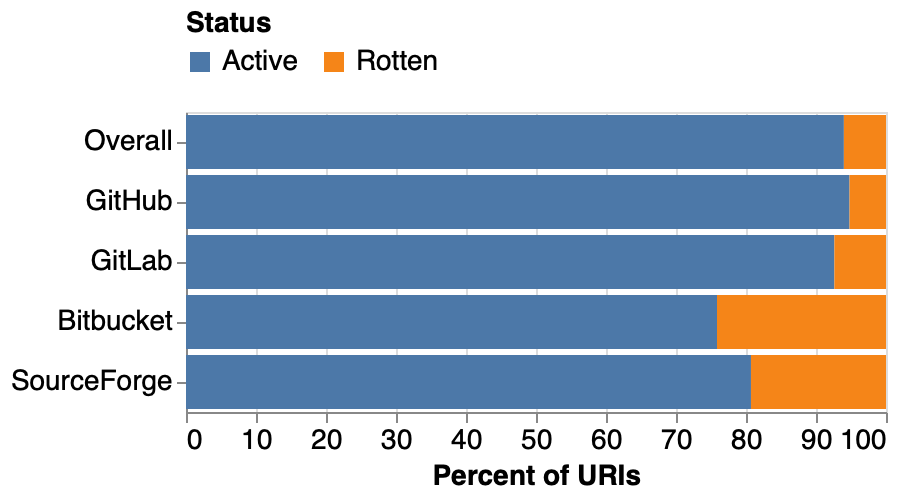
\includegraphics[width=0.95\linewidth]{is_it_alive_short.png}
    \caption{Percent of active URIs}
    \label{fig:alive}
\end{subfigure}
\begin{subfigure}{0.8\textwidth}
    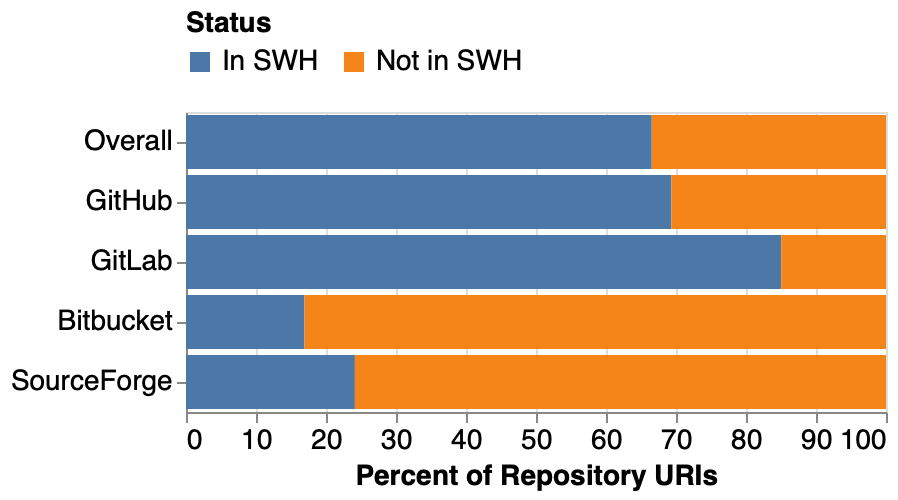
\includegraphics[width=0.95\linewidth]{is_it_in_swh_short.png}
    \caption{Percent of repository URIs captured by Software Heritage (SWH)}
    \label{fig:swh}
\end{subfigure}
% \end{figure}
% \begin{figure}\ContinuedFloat
% \centering
\begin{subfigure}{0.8\textwidth}
    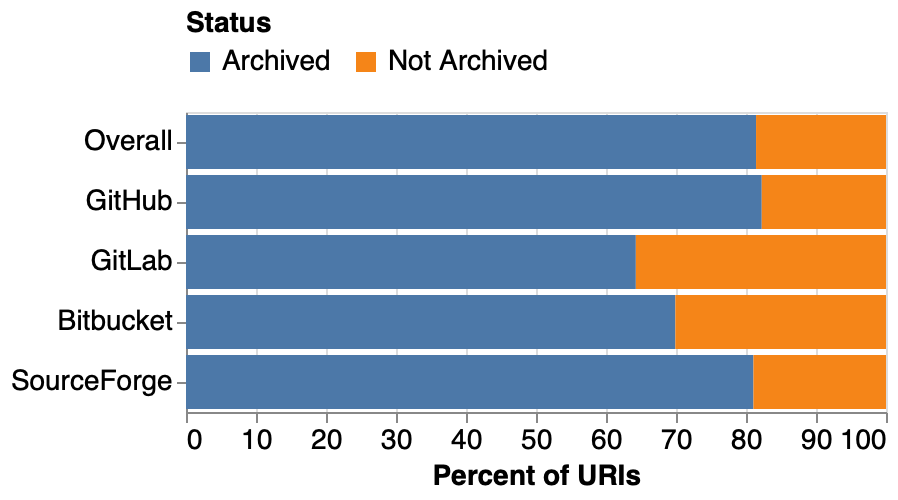
\includegraphics[width=0.95\linewidth]{is_it_archived_short.png}
    \caption{Percent of URIs that had at least one memento}
    \label{fig:timemap}
\end{subfigure}
\caption{Results of running the three tests: (1) is the URI active?, (2) has the URI been archived by Software Heritage?, and (3) has the URI been archived by Web archives?}
\label{fig:is_it}
\end{figure}

As shown in Figure \ref{fig:swh}, 62.07\% of all repository-level GHP URIs have at least one snapshot in Software Heritage. GitLab had the highest percentage of repository URIs captured by Software Heritage with 83.76\%. Bitbucket and SourceForge both have a relatively small percentage of repository URIs available in Software Heritage. Bitbucket had the lowest percentage with 15.87\% followed by SourceForge with 24.03\%

Across all four GHPs, 79.15\% of GHP URIs have at least one memento in the Web archives queried by MemGator, as shown in Figure \ref{fig:timemap}. GitHub had the highest percentage of URIs available in Web archives with 79.56\% and SourceForge was a close second with 79.01\%. GitLab had the smallest percentages of URIs available in Web archives with 62.51\%. The distribution of the percent of mementos returned from each of the twelve Web archives is shown in Table \ref{tab:archives}. Internet Archive had the largest percent of all returned mementos with 58.68\%. Internet Archive is followed by Bibliotheca Alexandrina Web Archive,\footnote{\url{https://www.bibalex.org/isis/frontend/archive/archive\_web.aspx}} which returned 23.29\% of all mementos. However, we note that since 2022 Bibliotheca Alexandrina has functioned as a backup to the Internet Archive and provides a mirror of the Internet Archive's holdings \cite{bibalex-ia}. %\footnote{https://www.bibalex.org/en/project/details?documentid=283}. 
This could explain the high percentage of GHP URIs available in both the Internet Archive and Bibliotheca Alexandrina Web archives. The remaining 18.03\% of mementos are distributed across the remaining 10 Web archives. 

\begin{table}
    \centering
    \begin{tabular}{|l|c|}
    \hline
    Web Archive & Percent of Mementos \\
    \hline
    Internet Archive & 58.68\% \\
    Bibliotheca Alexandria Web Archive & 23.29\% \\
    Archive.today & 8.06\% \\
    Archive.it & 3.07\% \\
    Portuguese Web Archive & 2.83\% \\
    Library of Congress & 2.53\% \\
    Icelandic Web Archive & 0.88\% \\
    Australian Web Archive & 0.35\% \\
    UK Web Archive & 0.12\% \\
    Perma & 0.11\% \\
    Stanford Web Archive & 0.08\% \\
    BAnQ & 0.0005\% (1 URI-M) \\ \hline
    \end{tabular}
    \caption{Percent of all mementos returned from each of the 12 Web archives}% queried by MemGator}
    \label{tab:archives}
\end{table}

% All of the statistics shown in Figure \ref{fig:is_it} are summarized in Table \ref{tab:stats}.

% \begin{table}
% \centering
% \begin{tabular}{|c|c|c|c|}
% \hline
%             & \multicolumn{3}{c|}{Percent of URIs available in} \\ \hline
% GHP         & Live Web      & SWH          & Web archives      \\ \hline
% Overall     & 93.62\%       & 62.06\%      & 79.15\%           \\ 
% GitHub      & 94.52\%       & 63.15\%      & 79.56\%           \\ 
% GitLab      & 89.38\%       & 83.76\%      & 62.51\%           \\ 
% Bitbucket   & 75.75\%       & 15.87\%      & 69.20\%           \\ 
% SourceForge & 80.14\%       & 24.03\%      & 79.01\%           \\
% \hline     
%     \end{tabular}
%     \caption{The percent of URIs that were active, archived by Software Heritage, and archived by Web archives for all URIs and for each of GHP}
%     \label{tab:stats}
% \end{table}

Figure \ref{fig:who_has_a_copy} depicts the percent of URIs archived by both Software Heritage and Web archives, only Software Heritage, only Web archives, and neither Software Heritage or Web archives. Overall, 54.46\% (68,330 URIs) of all URIs were captured by both Software Heritage and Web archives and 13.29\% (16,672 URIs) were not captured by either Software Heritage or the Web archives, making their resources unrecoverable. Across all four GHPs, there are a higher percentage of GHP URIs that have only been archived by Web archives (27.45\%) than the percentage of GHP URIs that have only been archived by Software Heritage (4.81\%). Source Forge and Bitbucket have the highest percentage of URIs unique to the Web archives with 63.96\% of SourceForge URIs 55.56\% of Bitbucket URIs only archived by Web archives. Bitbucket has the highest percentage of unrecoverable URI resources with 29.35\%. Figures \ref{fig:gh_sankey} and \ref{fig:bb_sankey} give a more detailed look at the relationship between each category for GitHub and Bitbucket URIs.  

\begin{figure}
\centering
\begin{subfigure}{0.9\textwidth}
    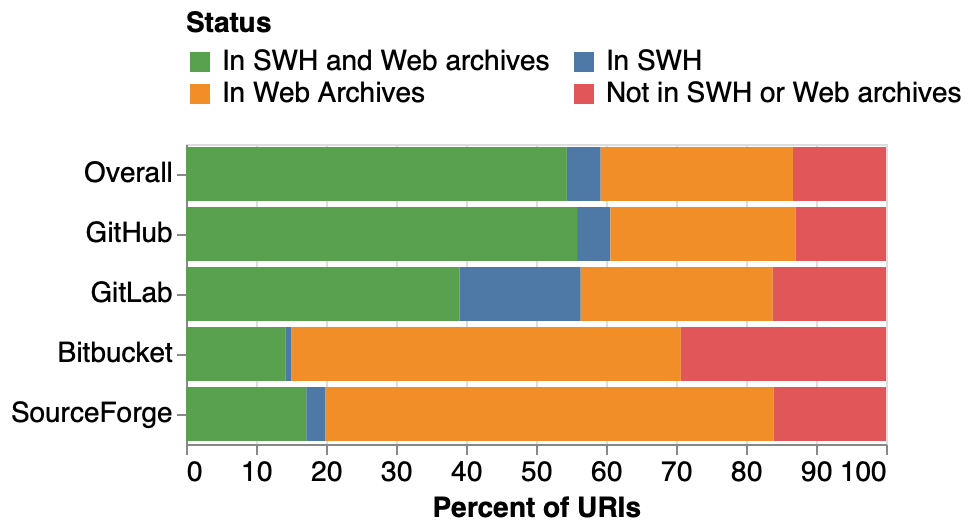
\includegraphics[width=0.95\linewidth]{who_has_a_copy_short.png}
    \caption{Percent of repository-level URIs overall and for each GHP}
    \label{fig:who_has_a_copy}
\end{subfigure}
%\end{figure}
%\begin{figure}%\ContinuedFloat
%\centering
\begin{subfigure}{0.9\textwidth}
    \centering
    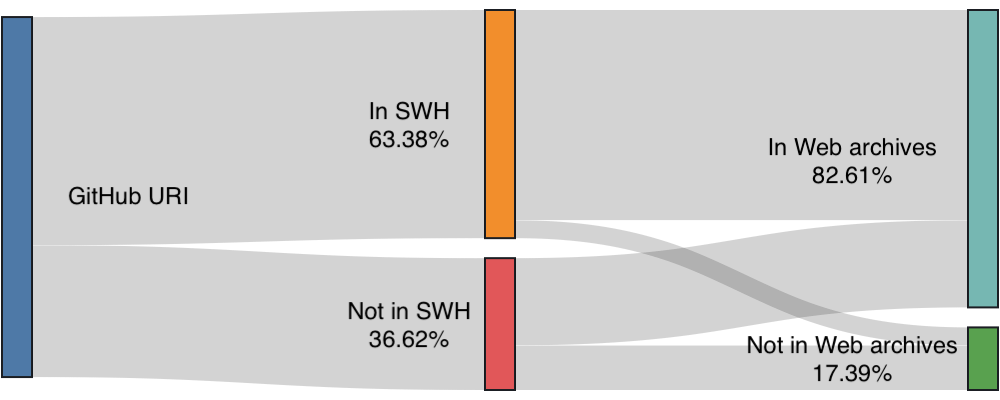
\includegraphics[width=0.95\linewidth]{gh_uri_chart.png}
    \caption{Relationship between the number of GitHub URIs preserved}
    \label{fig:gh_sankey}
\end{subfigure}
\begin{subfigure}{0.9\textwidth}
    \centering
    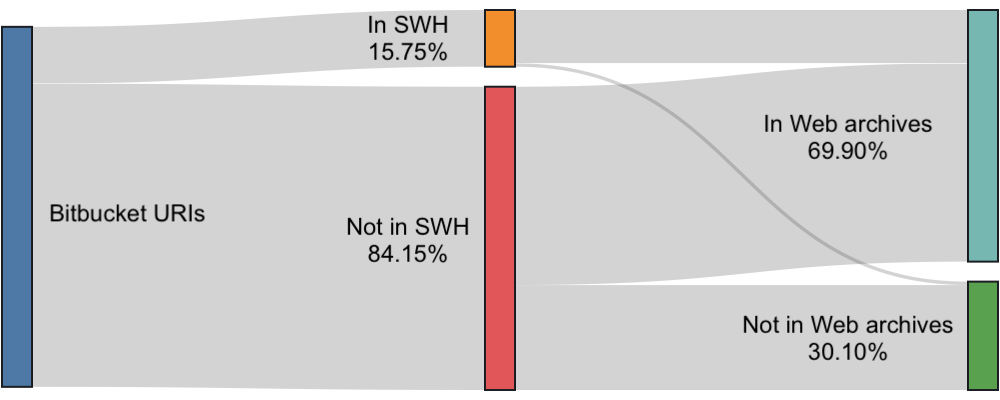
\includegraphics[width=0.95\linewidth]{bb_uri_chart.png}
    \caption{Relationship between the number of Bitbucket URIs preserved}
    \label{fig:bb_sankey}
\end{subfigure}
\caption{Relationships between URIs that have been archived by Software Heritage (SWH) and Web archives, only Software Heritage, only Web archives, and neither Software Heritage or Web archives}
\end{figure}

As shown in Figure \ref{fig:gh_sankey}, 58.24\% of GitHub URIs have been archived by both Software Heritage and Web archives, while 24.45\% of GitHub URIs have only been archived by Web archives. These percentages noticeably differ from the distribution of Bitbucket URIs as depicted in Figure 
\ref{fig:bb_sankey}. Of all Bitbucket URIs, 14.80\% have been archived by both Software Heritage and Web archives while 55.02\% have only been archived by Web archives. Additionally, only 0.95\% of Bitbucket URIs are archived by Software Heritage and not archived by Web archives, compared to 4.94\% of GitHub URIs. 

Because they have active URIs, vulnerable resources still have the opportunity to be archived by Web archives and Software Heritage. However, rotten URIs are no longer able to be preserved. Figure \ref{fig:dead_and_gone} depicts the percent of rotten URIs that have been archived by both Software Heritage and Web archives, only Software Heritage, only Web archives, and neither Software Heritage or Web archives. Across all four GHPs, 6,494 repository-level URIs are rotten and 37.20\% of rotten URIs are unrecoverable, as they have not been archived by Software Heritage or Web archives. In total, there are 2,416 unrecoverable URI resources across all four GHPs. GitLab has the smallest percentage of rotten URIs that have been archived by both Software Heritage and Web archives with 8.26\%. Conversely, Bitbucket has the largest percentage of rotten URIs that are captured by both Software Heritage and Web archives with 48.91\%. For rotten URIs, there is a smaller percentage of URIs that have only been archived by Software Heritage (8.18\%) than the percentage of URIs that have only been archived by Web archives (30.26\%). This trend is similar to what we saw for all GHP URIs in Figure \ref{fig:who_has_a_copy}. Figures \ref{fig:gh_dead_sankey} and \ref{fig:bb_dead_sankey} provide a more detailed look at the relationship between each category for rotten GitHub and Bitbucket URIs. 

\begin{figure}
\centering
\begin{subfigure}{0.8\textwidth}
    \centering
    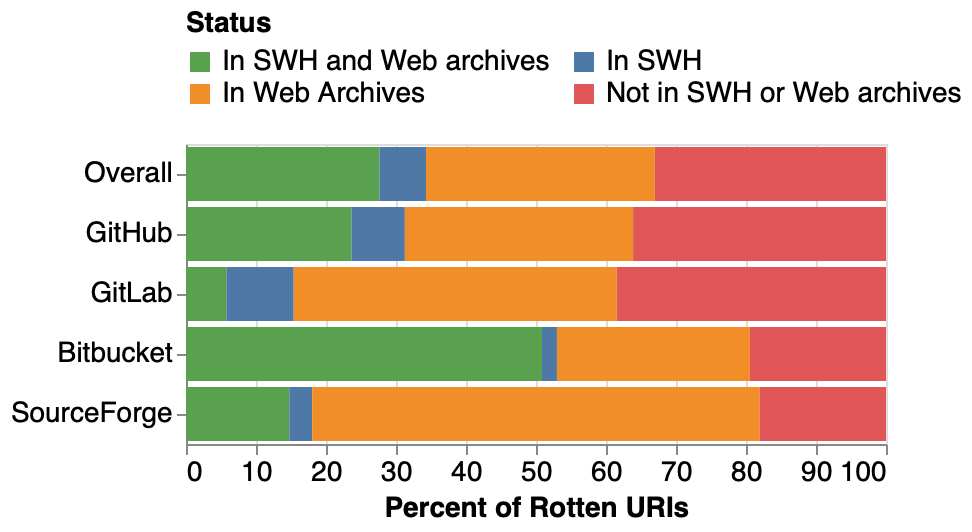
\includegraphics[width=\linewidth]{dead_and_gone_short.png}
    \caption{Percent of rotten repository-level URIs overall and for each GHP}
    \label{fig:dead_and_gone}
\end{subfigure}
%\end{figure}
%\begin{figure}%\ContinuedFloat
\centering
\begin{subfigure}{0.8\textwidth}
    \centering
    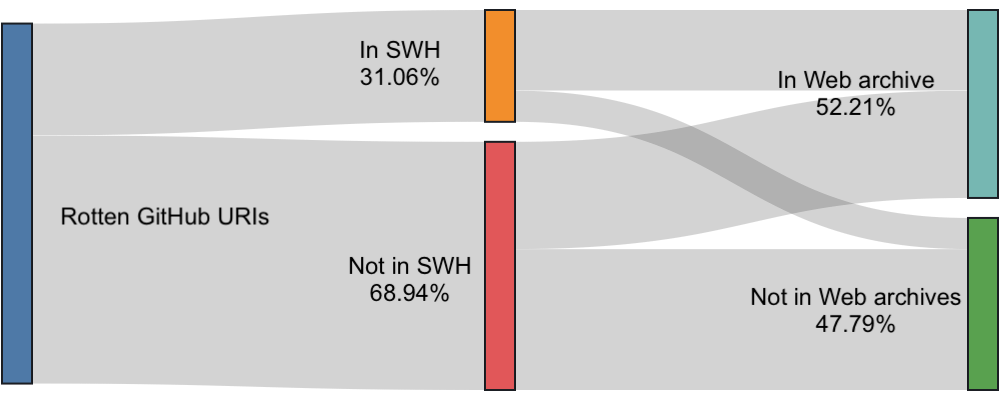
\includegraphics[width=\linewidth]{gh_dead_uri_chart.png}
    \caption{Preservation of rotten GitHub URIs}
    \label{fig:gh_dead_sankey}
\end{subfigure}
\begin{subfigure}{0.8\textwidth}
    \centering
    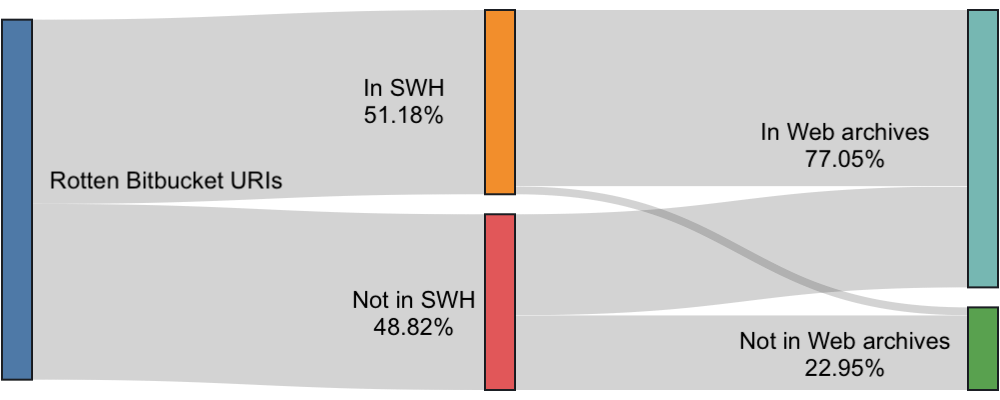
\includegraphics[width=\linewidth]{bb_dead_uri_chart.png}
    \caption{Preservation of rotten Bitbucket URIs}
    \label{fig:bb_dead_sankey}
\end{subfigure}
\caption{Relationships between rotten URIs that have been archived by Software Heritage (SWH) and Web archives, only Software Heritage, only Web archives, and neither Software Heritage or Web archives}
\end{figure}

As shown in Figure \ref{fig:gh_dead_sankey}, 47.76\% of rotten GitHub URIs are unrecoverable. Inversely, 22.37\% of rotten GitHub URIs have been archived by both Software Heritage and Web archives. GitHub has a larger percentage of rotten URIs that have only been archived by Software Heritage (8.66\%) than Bitbucket (2.18\%) as shown in Figure \ref{fig:bb_dead_sankey}. Again, the distribution of rotten Bitbucket URIs is distinguishable from the distribution of rotten GitHub URIs. We found that 20.73\% of rotten Bitbucket URIs are unrecoverable while 48.91\% of rotten Bitbucket URIs have been archived by both Software Heritage and Web archives.  

For both Software Heritage and Web archives, we calculated the time between the date of the first publication to reference a URI and the date of the first capture of the URI. Software Heritage was created on June 30, 2016 \cite{dicosmo_swhblog}, so we only analyzed articles that were published starting July 1, 2016. We found an average of 443 days (median of 360 days) between the first reference to the repository URI in a scholarly publication and the first capture by Software Heritage, if the repository-level URI did not have a snapshot at the time of publication. Additionally, 7,440 repository URIs that were captured before the publication date of the referencing article had not been captured since the article's publication. For these  URIs, there is an average of 253 days between the last Software Heritage snapshot and the publication date of the reference article. 

As shown in Figure \ref{fig:swh_delta},
the maximum time delta between the first reference to the repository URI in a scholarly publication and the first capture by Software Heritage has steadily decreased from 78 months for articles published in July 2016 to 9 months for articles published in April 2022. We also see that the median time delta follows a trend similar to the average time delta. The median and average time deltas have both decreased since 2021. 

\begin{figure}
    \centering
    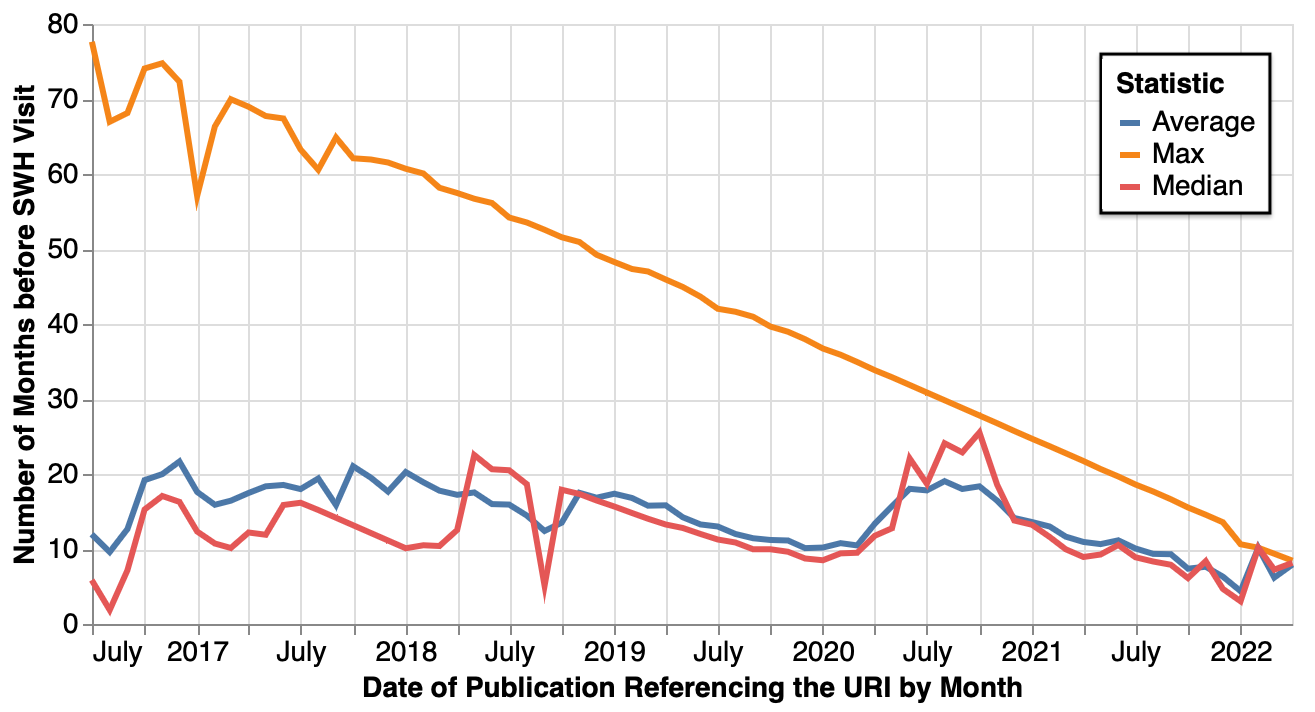
\includegraphics[width=0.85\linewidth]{SWH_delta_over_time.png}
    \caption{Months between a publication referencing a URI and the URI being captured by Software Heritage over time. Only includes URIs not been captured by Software Heritage before the publication date of the referencing article.}
    \label{fig:swh_delta}
\end{figure}

These trends for are similar for Web archives. There was an average of 468 days and a median of 341 days between the first reference to the URI in a scholarly publication and the first memento in a Web archive, if there were no mementos of the URI prior to the publication date of the referencing article. Of the URIs that had a memento in the Web archives prior to the publication date of the article, 4,356 URIs have not been archived since the article was published, with an average of 201 days between the latest memento and the publication date. Figure \ref{fig:timemap_delta} shows that the average and maximum time deltas have followed similar trends. Additionally, the maximum time delta has steadily decreased from 128 months in January 2012 to 1 month in April 2022. While the steady decline seen in maximum and average time deltas for Software Heritage and Web archives is promising, there is still a large period of time for the URI resource to move from  vulnerable to unrecoverable before Software Heritage or Web archives are able to archive it.

\begin{figure}
    \centering
    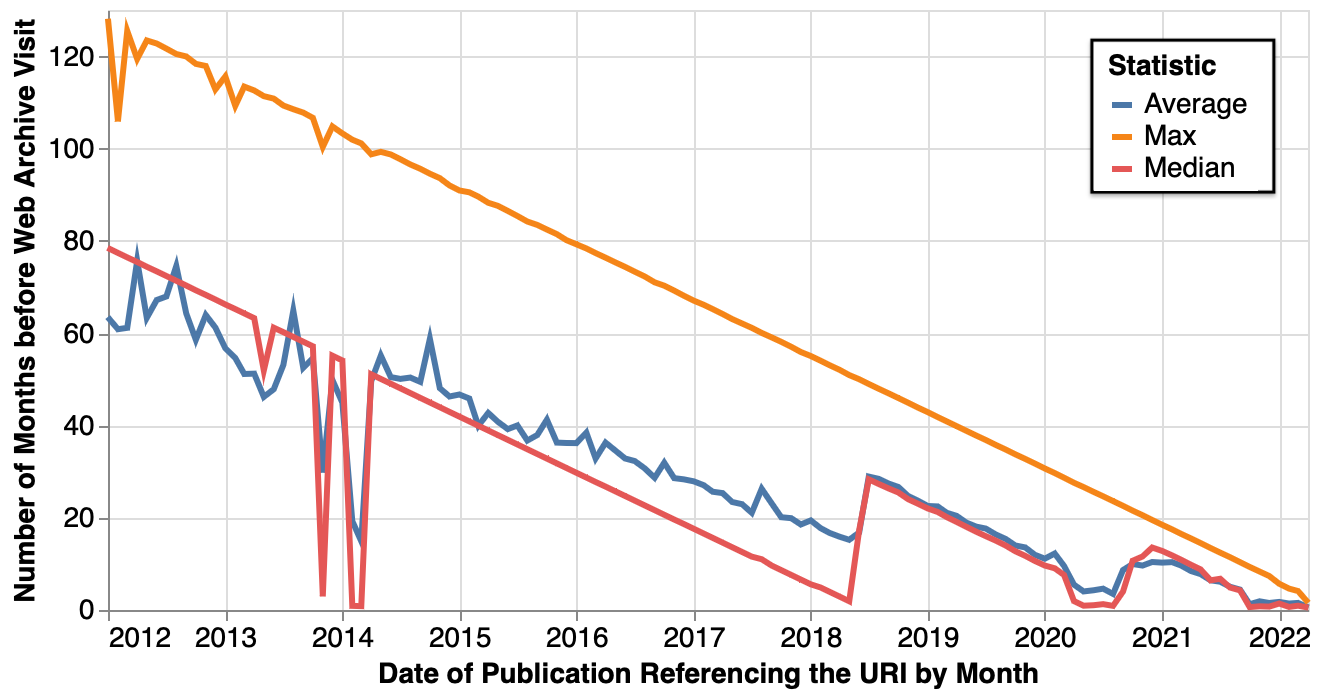
\includegraphics[width=0.85\linewidth]{archives_delta_over_time.png}
    \caption{Number of months between a publication referencing a URI and the URI being captured by the Web archives over time. Only includes URIs not captured by the Web archives before the publication date of the referencing article.}
    \label{fig:timemap_delta}
\end{figure}